


\tikzset{every picture/.style={line width=0.75pt}} %set default line width to 0.75pt        

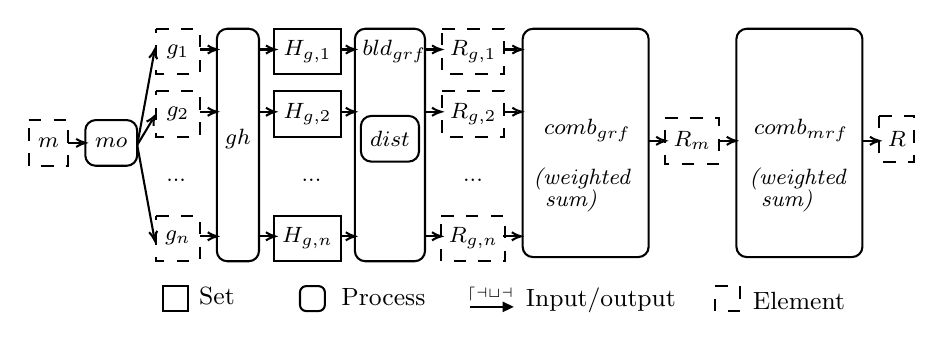
\begin{tikzpicture}[x=0.75pt,y=0.75pt,yscale=-1,xscale=1]
%uncomment if require: \path (0,2218); %set diagram left start at 0, and has height of 2218

%Shape: Rectangle [id:dp13808213408235837] 
\draw   (284.45,1997) .. controls (284.45,1994.24) and (286.69,1992) .. (289.45,1992) -- (313.25,1992) .. controls (316.02,1992) and (318.25,1994.24) .. (318.25,1997) -- (318.25,2099) .. controls (318.25,2101.76) and (316.02,2104) .. (313.25,2104) -- (289.45,2104) .. controls (286.69,2104) and (284.45,2101.76) .. (284.45,2099) -- cycle ;
%Shape: Rectangle [id:dp74308620499086] 
\draw   (365.28,1997) .. controls (365.28,1994.24) and (367.52,1992) .. (370.28,1992) -- (421,1992) .. controls (423.76,1992) and (426,1994.24) .. (426,1997) -- (426,2097) .. controls (426,2099.76) and (423.76,2102) .. (421,2102) -- (370.28,2102) .. controls (367.52,2102) and (365.28,2099.76) .. (365.28,2097) -- cycle ;
%Shape: Rectangle [id:dp9492596901861552] 
\draw   (217.94,1997) .. controls (217.94,1994.24) and (220.18,1992) .. (222.94,1992) -- (233.27,1992) .. controls (236.03,1992) and (238.27,1994.24) .. (238.27,1997) -- (238.27,2099) .. controls (238.27,2101.76) and (236.03,2104) .. (233.27,2104) -- (222.94,2104) .. controls (220.18,2104) and (217.94,2101.76) .. (217.94,2099) -- cycle ;
%Straight Lines [id:da2889666579464296] 
\draw    (179.59,2048) -- (187.68,2003.97) ;
\draw [shift={(188.04,2002)}, rotate = 100.41] [color={rgb, 255:red, 0; green, 0; blue, 0 }  ][line width=0.75]    (4.37,-1.96) .. controls (2.78,-0.92) and (1.32,-0.27) .. (0,0) .. controls (1.32,0.27) and (2.78,0.92) .. (4.37,1.96)   ;
%Straight Lines [id:da29295133800326556] 
\draw    (179.59,2048) -- (187.68,2092.03) ;
\draw [shift={(188.04,2094)}, rotate = 259.59] [color={rgb, 255:red, 0; green, 0; blue, 0 }  ][line width=0.75]    (4.37,-1.96) .. controls (2.78,-0.92) and (1.32,-0.27) .. (0,0) .. controls (1.32,0.27) and (2.78,0.92) .. (4.37,1.96)   ;
%Straight Lines [id:da3918782953792337] 
\draw    (179.59,2048) -- (187,2035.71) ;
\draw [shift={(188.04,2034)}, rotate = 121.12] [color={rgb, 255:red, 0; green, 0; blue, 0 }  ][line width=0.75]    (4.37,-1.96) .. controls (2.78,-0.92) and (1.32,-0.27) .. (0,0) .. controls (1.32,0.27) and (2.78,0.92) .. (4.37,1.96)   ;
%Straight Lines [id:da48722664363967816] 
\draw    (209.69,2002) -- (215.94,2002) ;
\draw [shift={(217.94,2002)}, rotate = 180] [color={rgb, 255:red, 0; green, 0; blue, 0 }  ][line width=0.75]    (4.37,-1.96) .. controls (2.78,-0.92) and (1.32,-0.27) .. (0,0) .. controls (1.32,0.27) and (2.78,0.92) .. (4.37,1.96)   ;
%Straight Lines [id:da19690491748144945] 
\draw    (209.69,2032) -- (215.94,2032) ;
\draw [shift={(217.94,2032)}, rotate = 180] [color={rgb, 255:red, 0; green, 0; blue, 0 }  ][line width=0.75]    (4.37,-1.96) .. controls (2.78,-0.92) and (1.32,-0.27) .. (0,0) .. controls (1.32,0.27) and (2.78,0.92) .. (4.37,1.96)   ;
%Straight Lines [id:da5862338360201571] 
\draw    (209.69,2092) -- (215.94,2092) ;
\draw [shift={(217.94,2092)}, rotate = 180] [color={rgb, 255:red, 0; green, 0; blue, 0 }  ][line width=0.75]    (4.37,-1.96) .. controls (2.78,-0.92) and (1.32,-0.27) .. (0,0) .. controls (1.32,0.27) and (2.78,0.92) .. (4.37,1.96)   ;
%Straight Lines [id:da31052528835050563] 
\draw    (238.27,2002) -- (244,2002) ;
\draw [shift={(246,2002)}, rotate = 180] [color={rgb, 255:red, 0; green, 0; blue, 0 }  ][line width=0.75]    (4.37,-1.96) .. controls (2.78,-0.92) and (1.32,-0.27) .. (0,0) .. controls (1.32,0.27) and (2.78,0.92) .. (4.37,1.96)   ;
%Straight Lines [id:da6932670362664344] 
\draw    (238.27,2032) -- (244,2032) ;
\draw [shift={(246,2032)}, rotate = 180] [color={rgb, 255:red, 0; green, 0; blue, 0 }  ][line width=0.75]    (4.37,-1.96) .. controls (2.78,-0.92) and (1.32,-0.27) .. (0,0) .. controls (1.32,0.27) and (2.78,0.92) .. (4.37,1.96)   ;
%Straight Lines [id:da8977162967633212] 
\draw    (238.27,2092) -- (244,2092) ;
\draw [shift={(246,2092)}, rotate = 180] [color={rgb, 255:red, 0; green, 0; blue, 0 }  ][line width=0.75]    (4.37,-1.96) .. controls (2.78,-0.92) and (1.32,-0.27) .. (0,0) .. controls (1.32,0.27) and (2.78,0.92) .. (4.37,1.96)   ;
%Straight Lines [id:da6122296788133859] 
\draw    (278.11,2002) -- (282.45,2002) ;
\draw [shift={(284.45,2002)}, rotate = 180] [color={rgb, 255:red, 0; green, 0; blue, 0 }  ][line width=0.75]    (4.37,-1.96) .. controls (2.78,-0.92) and (1.32,-0.27) .. (0,0) .. controls (1.32,0.27) and (2.78,0.92) .. (4.37,1.96)   ;
%Straight Lines [id:da5829648880002971] 
\draw    (278.11,2032) -- (282.45,2032) ;
\draw [shift={(284.45,2032)}, rotate = 180] [color={rgb, 255:red, 0; green, 0; blue, 0 }  ][line width=0.75]    (4.37,-1.96) .. controls (2.78,-0.92) and (1.32,-0.27) .. (0,0) .. controls (1.32,0.27) and (2.78,0.92) .. (4.37,1.96)   ;
%Straight Lines [id:da513713543311537] 
\draw    (278.11,2092) -- (282.45,2092) ;
\draw [shift={(284.45,2092)}, rotate = 180] [color={rgb, 255:red, 0; green, 0; blue, 0 }  ][line width=0.75]    (4.37,-1.96) .. controls (2.78,-0.92) and (1.32,-0.27) .. (0,0) .. controls (1.32,0.27) and (2.78,0.92) .. (4.37,1.96)   ;
%Straight Lines [id:da6438386079044336] 
\draw    (318.25,2002) -- (324,2002) ;
\draw [shift={(326,2002)}, rotate = 180] [color={rgb, 255:red, 0; green, 0; blue, 0 }  ][line width=0.75]    (4.37,-1.96) .. controls (2.78,-0.92) and (1.32,-0.27) .. (0,0) .. controls (1.32,0.27) and (2.78,0.92) .. (4.37,1.96)   ;
%Straight Lines [id:da8785685038782167] 
\draw    (318.25,2032) -- (324,2032) ;
\draw [shift={(326,2032)}, rotate = 180] [color={rgb, 255:red, 0; green, 0; blue, 0 }  ][line width=0.75]    (4.37,-1.96) .. controls (2.78,-0.92) and (1.32,-0.27) .. (0,0) .. controls (1.32,0.27) and (2.78,0.92) .. (4.37,1.96)   ;
%Straight Lines [id:da41812553219121584] 
\draw    (318.25,2092) -- (324,2092) ;
\draw [shift={(326,2092)}, rotate = 180] [color={rgb, 255:red, 0; green, 0; blue, 0 }  ][line width=0.75]    (4.37,-1.96) .. controls (2.78,-0.92) and (1.32,-0.27) .. (0,0) .. controls (1.32,0.27) and (2.78,0.92) .. (4.37,1.96)   ;
%Straight Lines [id:da7655995227933847] 
\draw    (356.25,2002) -- (362.7,2002) ;
\draw [shift={(364.7,2002)}, rotate = 180] [color={rgb, 255:red, 0; green, 0; blue, 0 }  ][line width=0.75]    (4.37,-1.96) .. controls (2.78,-0.92) and (1.32,-0.27) .. (0,0) .. controls (1.32,0.27) and (2.78,0.92) .. (4.37,1.96)   ;
%Straight Lines [id:da18029052337035645] 
\draw    (356.25,2032) -- (362.7,2032) ;
\draw [shift={(364.7,2032)}, rotate = 180] [color={rgb, 255:red, 0; green, 0; blue, 0 }  ][line width=0.75]    (4.37,-1.96) .. controls (2.78,-0.92) and (1.32,-0.27) .. (0,0) .. controls (1.32,0.27) and (2.78,0.92) .. (4.37,1.96)   ;
%Straight Lines [id:da7858238392262193] 
\draw    (356,2092) -- (362.45,2092) ;
\draw [shift={(364.45,2092)}, rotate = 180] [color={rgb, 255:red, 0; green, 0; blue, 0 }  ][line width=0.75]    (4.37,-1.96) .. controls (2.78,-0.92) and (1.32,-0.27) .. (0,0) .. controls (1.32,0.27) and (2.78,0.92) .. (4.37,1.96)   ;
%Straight Lines [id:da7686017918442807] 
\draw    (426,2046) -- (432,2046) ;
\draw [shift={(434,2046)}, rotate = 180] [color={rgb, 255:red, 0; green, 0; blue, 0 }  ][line width=0.75]    (4.37,-1.96) .. controls (2.78,-0.92) and (1.32,-0.27) .. (0,0) .. controls (1.32,0.27) and (2.78,0.92) .. (4.37,1.96)   ;
%Shape: Rectangle [id:dp664345223446329] 
\draw   (468.27,1997) .. controls (468.27,1994.24) and (470.51,1992) .. (473.27,1992) -- (523.99,1992) .. controls (526.75,1992) and (528.99,1994.24) .. (528.99,1997) -- (528.99,2097) .. controls (528.99,2099.76) and (526.75,2102) .. (523.99,2102) -- (473.27,2102) .. controls (470.51,2102) and (468.27,2099.76) .. (468.27,2097) -- cycle ;
%Straight Lines [id:da879639811758731] 
\draw    (460,2046) -- (466,2046) ;
\draw [shift={(468,2046)}, rotate = 180] [color={rgb, 255:red, 0; green, 0; blue, 0 }  ][line width=0.75]    (4.37,-1.96) .. controls (2.78,-0.92) and (1.32,-0.27) .. (0,0) .. controls (1.32,0.27) and (2.78,0.92) .. (4.37,1.96)   ;
%Straight Lines [id:da7919453986075877] 
\draw    (529,2046) -- (535,2046) ;
\draw [shift={(537,2046)}, rotate = 180] [color={rgb, 255:red, 0; green, 0; blue, 0 }  ][line width=0.75]    (4.37,-1.96) .. controls (2.78,-0.92) and (1.32,-0.27) .. (0,0) .. controls (1.32,0.27) and (2.78,0.92) .. (4.37,1.96)   ;
%Shape: Rectangle [id:dp9877761412973047] 
\draw  [fill={rgb, 255:red, 255; green, 255; blue, 255 }  ,fill opacity=1 ] (192,2116) -- (204,2116) -- (204,2128) -- (192,2128) -- cycle ;
%Shape: Rectangle [id:dp5934748209836505] 
\draw  [fill={rgb, 255:red, 255; green, 255; blue, 255 }  ,fill opacity=1 ] (258,2119) .. controls (258,2117.34) and (259.34,2116) .. (261,2116) -- (267,2116) .. controls (268.66,2116) and (270,2117.34) .. (270,2119) -- (270,2125) .. controls (270,2126.66) and (268.66,2128) .. (267,2128) -- (261,2128) .. controls (259.34,2128) and (258,2126.66) .. (258,2125) -- cycle ;
%Straight Lines [id:da8694977414056682] 
\draw    (340,2126) -- (358,2126) ;
\draw [shift={(361,2126)}, rotate = 180] [fill={rgb, 255:red, 0; green, 0; blue, 0 }  ][line width=0.08]  [draw opacity=0] (5.36,-2.57) -- (0,0) -- (5.36,2.57) -- cycle    ;
%Shape: Rectangle [id:dp3381818681548523] 
\draw  [fill={rgb, 255:red, 255; green, 255; blue, 255 }  ,fill opacity=1 ][dash pattern={on 4.5pt off 4.5pt}] (458,2116) -- (470,2116) -- (470,2128) -- (458,2128) -- cycle ;

% Text Node
\draw  [dash pattern={on 4.5pt off 4.5pt}]  (326.5,1992) -- (356.5,1992) -- (356.5,2014) -- (326.5,2014) -- cycle  ;
\draw (341.5,2003) node  [font=\footnotesize] [align=left] {$\displaystyle R_{g,1}$};
% Text Node
\draw (303.47,2003) node  [font=\footnotesize] [align=left] {$\displaystyle bld_{grf}$};
% Text Node
\draw (396.5,2041) node  [font=\footnotesize] [align=left] {$\displaystyle comb_{grf}$};
% Text Node
\draw    (154.57,2041) .. controls (154.57,2038.24) and (156.81,2036) .. (159.57,2036) -- (174.57,2036) .. controls (177.33,2036) and (179.57,2038.24) .. (179.57,2041) -- (179.57,2053) .. controls (179.57,2055.76) and (177.33,2058) .. (174.57,2058) -- (159.57,2058) .. controls (156.81,2058) and (154.57,2055.76) .. (154.57,2053) -- cycle  ;
\draw (167.07,2047) node  [font=\footnotesize] [align=left] {$\displaystyle mo$};
% Text Node
\draw    (287.35,2039) .. controls (287.35,2036.24) and (289.59,2034) .. (292.35,2034) -- (310.35,2034) .. controls (313.11,2034) and (315.35,2036.24) .. (315.35,2039) -- (315.35,2051) .. controls (315.35,2053.76) and (313.11,2056) .. (310.35,2056) -- (292.35,2056) .. controls (289.59,2056) and (287.35,2053.76) .. (287.35,2051) -- cycle  ;
\draw (301.35,2045) node  [font=\footnotesize] [align=left] {$\displaystyle dist$};
% Text Node
\draw  [dash pattern={on 4.5pt off 4.5pt}]  (537,2034) -- (554,2034) -- (554,2056) -- (537,2056) -- cycle  ;
\draw (545.5,2045) node  [font=\footnotesize] [align=left] {$\displaystyle R$};
% Text Node
\draw  [dash pattern={on 4.5pt off 4.5pt}]  (434,2035) -- (460,2035) -- (460,2057) -- (434,2057) -- cycle  ;
\draw (447,2046) node  [font=\footnotesize] [align=left] {$\displaystyle R_{m}$};
% Text Node
\draw  [dash pattern={on 4.5pt off 4.5pt}]  (326.5,2022) -- (356.5,2022) -- (356.5,2044) -- (326.5,2044) -- cycle  ;
\draw (341.5,2033) node  [font=\footnotesize] [align=left] {$\displaystyle R_{g,2}$};
% Text Node
\draw  [dash pattern={on 4.5pt off 4.5pt}]  (326,2082) -- (357,2082) -- (357,2104) -- (326,2104) -- cycle  ;
\draw (341.5,2093) node  [font=\footnotesize] [align=left] {$\displaystyle R_{g,n}$};
% Text Node
\draw (341.37,2065) node  [font=\footnotesize] [align=left] {$\displaystyle ...$};
% Text Node
\draw    (245.61,1992) -- (277.61,1992) -- (277.61,2014) -- (245.61,2014) -- cycle  ;
\draw (261.61,2003) node  [font=\footnotesize] [align=left] {$\displaystyle H_{g,1}$};
% Text Node
\draw    (245.61,2022) -- (277.61,2022) -- (277.61,2044) -- (245.61,2044) -- cycle  ;
\draw (261.61,2033) node  [font=\footnotesize] [align=left] {$\displaystyle H_{g,2}$};
% Text Node
\draw    (245.61,2082) -- (277.61,2082) -- (277.61,2104) -- (245.61,2104) -- cycle  ;
\draw (261.61,2093) node  [font=\footnotesize] [align=left] {$\displaystyle H_{g,n}$};
% Text Node
\draw (263.56,2065) node  [font=\footnotesize] [align=left] {$\displaystyle ...$};
% Text Node
\draw  [dash pattern={on 4.5pt off 4.5pt}]  (127.31,2036) -- (146.31,2036) -- (146.31,2058) -- (127.31,2058) -- cycle  ;
\draw (136.81,2047) node  [font=\footnotesize] [align=left] {$\displaystyle m$};
% Text Node
\draw  [dash pattern={on 4.5pt off 4.5pt}]  (188.69,1992) -- (209.69,1992) -- (209.69,2014) -- (188.69,2014) -- cycle  ;
\draw (199.19,2003) node  [font=\footnotesize] [align=left] {$\displaystyle g_{1}$};
% Text Node
\draw  [dash pattern={on 4.5pt off 4.5pt}]  (188.69,2022) -- (209.69,2022) -- (209.69,2044) -- (188.69,2044) -- cycle  ;
\draw (199.19,2033) node  [font=\footnotesize] [align=left] {$\displaystyle g_{2}$};
% Text Node
\draw  [dash pattern={on 4.5pt off 4.5pt}]  (188.69,2082) -- (209.69,2082) -- (209.69,2104) -- (188.69,2104) -- cycle  ;
\draw (199.19,2093) node  [font=\footnotesize] [align=left] {$\displaystyle g_{n}$};
% Text Node
\draw (198.38,2065) node  [font=\footnotesize] [align=left] {$\displaystyle ...$};
% Text Node
\draw (228.1,2045) node  [font=\footnotesize] [align=left] {$\displaystyle gh$};
% Text Node
\draw (369,2055) node [anchor=north west][inner sep=0.75pt]  [font=\scriptsize] [align=left] {\begin{minipage}[lt]{27.42pt}\setlength\topsep{0pt}
\begin{center}
{\footnotesize \textit{(weighted}}\\{\footnotesize \textit{sum)}}
\end{center}

\end{minipage}};
% Text Node
\draw (499.49,2041) node  [font=\footnotesize] [align=left] {$\displaystyle comb_{mrf}$};
% Text Node
\draw (473,2055) node [anchor=north west][inner sep=0.75pt]  [font=\scriptsize] [align=left] {\begin{minipage}[lt]{27.42pt}\setlength\topsep{0pt}
\begin{center}
{\footnotesize \textit{(weighted}}\\{\footnotesize \textit{sum)}}
\end{center}

\end{minipage}};
% Text Node
\draw (218,2121) node  [font=\footnotesize] [align=left] {\begin{minipage}[lt]{13.75pt}\setlength\topsep{0pt}
\begin{center}
{\small Set}
\end{center}

\end{minipage}};
% Text Node
\draw (297.5,2119) node  [font=\footnotesize] [align=left] {\begin{minipage}[lt]{29.25pt}\setlength\topsep{0pt}
\begin{center}
{\small Process}
\end{center}

\end{minipage}};
% Text Node
\draw (394.5,2121) node  [font=\footnotesize] [align=left] {\begin{minipage}[lt]{41.51pt}\setlength\topsep{0pt}
\begin{center}
{\small Input/output}
\end{center}

\end{minipage}};
% Text Node
\draw (349.5,2120) node  [font=\tiny] [align=left] {$\displaystyle \mathcal{data}$};
% Text Node
\draw (496,2121) node  [font=\footnotesize] [align=left] {\begin{minipage}[lt]{29.65pt}\setlength\topsep{0pt}
\begin{center}
{\small Element}
\end{center}

\end{minipage}};
% Connection
\draw    (146.31,2047) -- (152.57,2047) ;
\draw [shift={(154.57,2047)}, rotate = 180] [color={rgb, 255:red, 0; green, 0; blue, 0 }  ][line width=0.75]    (4.37,-1.96) .. controls (2.78,-0.92) and (1.32,-0.27) .. (0,0) .. controls (1.32,0.27) and (2.78,0.92) .. (4.37,1.96)   ;

\end{tikzpicture}